% !TeX spellcheck = en_US

\begin{figure}
	\centering
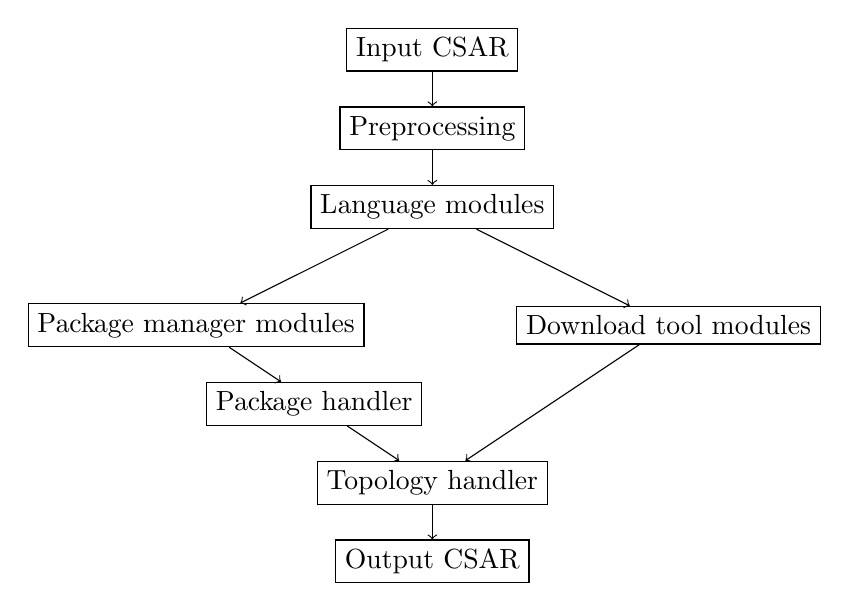
\begin{tikzpicture}
\node[draw] (in) at (0,1.5) {Input CSAR};
\node[draw] (pp) at (0,+0.5) {Preprocessing};
\node[draw] (lm) at (0,-0.5) {Language modules};
\node[draw] (pmm) at (-3,-2) {Package manager modules};
\node[draw] (dtm) at (+3,-2) {Download tool modules};
\node[draw] (ph) at (-1.5,-3) {Package handler};
\node[draw] (th) at (0,-4) {Topology handler};
\node[draw] (out) at (0,-5) {Output CSAR};
\draw [->] (in) -- (pp);
\draw [->] (pp) -- (lm);
\draw [->] (lm) -- (pmm);
\draw [->] (lm) -- (dtm);
\draw [->] (pmm) -- (ph);
\draw [->] (dtm) -- (th);
\draw [->] (ph) -- (th);
\draw [->] (th) -- (out);
\end{tikzpicture} 
\caption{The general description of the software's work flow} 	\label{fig:gen}
\end{figure}